% 07_economics_floats.tex -- tables and figures for this section (2026-10-15), each \input from a generated/ file or an
% \includegraphics of a generated figure; generators: writeup/make_rehaul_*.py. Placed after the section in paper_rehaul.tex
% so section text and floats can be edited in parallel; move them inline when the prose settles.
%
% Generator: writeup/make_rehaul_economics.py (outline 7.4: tables E1-E4 and three figures; it asserts the outline's
% headline numbers and gates every E1 statistic against results/close_master_table/master_table.csv). Prose macros
% \rhe... for 07_economics.tex: generated/rehaul_econ_numbers.tex (not \input here).
% Labels: tab:rh_econ_control (E1), tab:rh_econ_allfeat (E2), tab:rh_econ_pooled (E3), tab:rh_econ_sizing (E4),
% fig:rh_econ_cumpnl, fig:rh_econ_qlike_sharpe, fig:rh_econ_sizing, fig:rh_econ_byyear.
% Figure palette (one hue per family, also in the tables' panel order): per-bar linear blue, per-bar trees vermillion,
% per-bar MinGRU green, pooled magenta, always short black dashed. fig_qlike_sharpe keeps its own per-estimator colours.

% E1: always short and the key forecasts
% AUTO-GENERATED by writeup/make_rehaul_economics.py -- do not edit; re-run the script.
% Table E1 (outline 7.4): always short and the key forecasts under sign(s), 866 trade days.
\begin{table}[tbp]
\centering
\small
\setlength{\tabcolsep}{4.5pt}
\begin{threeparttable}
\caption{The closing trade under $q_t = \sign(s_t)$: always short and the key forecasts, 866 trade days.}
\label{tab:rh_econ_control}
\begin{tabular}{@{}lrrrrrrrr@{}}
\toprule
 & \multicolumn{2}{c}{Mid return} & \multicolumn{2}{c}{Sharpe ratio} & & & \multicolumn{2}{c}{vs always short} \\
\cmidrule(lr){2-3}\cmidrule(lr){4-5}\cmidrule(l){8-9}
Forecast & Mean (\%) & $t$ & Mid & Crossed & Hit (\%) & Buys (\%) & $\Delta$Sharpe & $t$ \\
\midrule
Always short ($q_t = -1$) & $1.4$ & $0.43$ & $0.20$ & $-0.27$ & $61.8$ & $0.0$ & -- & -- \\
\addlinespace[3pt]
\multicolumn{9}{@{}l}{\textit{Per-bar linear (16:00 bar)}} \\
OLS, HAR + calendar & {\bfseries\boldmath $9.7$} & {\bfseries\boldmath $2.83$} & $1.37$ & $0.89$ & $56.7$ & $27.9$ & $+1.17$ & $1.85$ \\
Elastic net, all features & {\bfseries\boldmath $13.5$} & {\bfseries\boldmath $3.66$} & $1.92$ & $1.43$ & $57.7$ & $28.3$ & {\bfseries\boldmath $+1.72$} & {\bfseries\boldmath $2.56$} \\
Lasso, all features & {\bfseries\boldmath $13.2$} & {\bfseries\boldmath $3.81$} & $1.88$ & $1.40$ & $57.6$ & $29.6$ & {\bfseries\boldmath $+1.67$} & {\bfseries\boldmath $2.54$} \\
Ridge, all features & {\bfseries\boldmath $10.0$} & {\bfseries\boldmath $2.86$} & $1.42$ & $0.93$ & $57.5$ & $27.1$ & {\bfseries\boldmath $+1.21$} & {\bfseries\boldmath $1.98$} \\
\addlinespace[3pt]
\multicolumn{9}{@{}l}{\textit{Per-bar trees, all features}} \\
LightGBM\tnote{a} & {\bfseries\boldmath $12.8$} & {\bfseries\boldmath $3.73$} & $1.81$ & $1.33$ & $56.9$ & $30.5$ & {\bfseries\boldmath $+1.61$} & {\bfseries\boldmath $2.33$} \\
XGBoost\tnote{a} & {\bfseries\boldmath $12.5$} & {\bfseries\boldmath $3.82$} & $1.77$ & $1.27$ & $58.7$ & $27.8$ & {\bfseries\boldmath $+1.56$} & {\bfseries\boldmath $2.56$} \\
Random forest\tnote{a} & {\bfseries\boldmath $11.2$} & {\bfseries\boldmath $3.38$} & $1.58$ & $1.11$ & $56.8$ & $30.4$ & {\bfseries\boldmath $+1.38$} & {\bfseries\boldmath $2.07$} \\
\addlinespace[3pt]
\multicolumn{9}{@{}l}{\textit{Per-bar neural net}} \\
MinGRU, all features\tnote{b} & {\bfseries\boldmath $10.8$} & {\bfseries\boldmath $3.09$} & $1.53$ & $1.05$ & $56.2$ & $32.8$ & {\bfseries\boldmath $+1.33$} & {\bfseries\boldmath $2.02$} \\
\addlinespace[3pt]
\multicolumn{9}{@{}l}{\textit{Pooled linear (all 48 bars)}} \\
Elastic net, all features & {\bfseries\boldmath $10.6$} & {\bfseries\boldmath $2.81$} & $1.50$ & $1.01$ & $57.3$ & $27.4$ & $+1.29$ & $1.90$ \\
Lasso, all features & {\bfseries\boldmath $8.5$} & {\bfseries\boldmath $2.45$} & $1.20$ & $0.71$ & $58.0$ & $23.7$ & $+1.00$ & $1.66$ \\
Ridge, all features & {\bfseries\boldmath $10.2$} & {\bfseries\boldmath $2.78$} & $1.44$ & $0.96$ & $57.5$ & $27.1$ & $+1.24$ & $1.93$ \\
\bottomrule
\end{tabular}
\begin{tablenotes}[flushleft]
\footnotesize
\item \textit{Notes:} One 0DTE SPXW straddle (a one-strike strangle when spot is between strikes) is bought
($q_t = +1$) or sold ($q_t = -1$) at 15:30 ET and held to the close; $r_t = q_t R_t$, with $R_t$ the return on the
premium; 3 January 2020 to 30 April 2024. Mid: the straddle is bought or sold at the 15:30 midpoint; crossed: a buy pays the ask and a sale receives the bid, the spread paid at entry only (settlement is cash at intrinsic). Mean: the mean mid return, in \% of the premium. Sharpe ratio $=\sqrt{252}\,\bar r/\mathrm{sd}(r)$, annualised per trade day (the trade runs about 200 days a year).
Hit: share of days with $r_t > 0$ at mid; Buys: share of days with $q_t = +1$. $\Delta$Sharpe: mid Sharpe ratio minus
always short's ($0.20$). Every $t$ is Newey--West (Bartlett kernel, lag $\lfloor 1.5\,n^{1/3}\rfloor = 14$ at $n = 866$); the $t$ of a $\Delta$Sharpe is that of the mean daily return difference, so it tests the mean difference, not the Sharpe difference. Bold: $|t| > 1.96$ (5\,\%, two-sided), on the estimate and its $t$.
\item[a] Of each estimator's 15 configurations on all features in the model set, the one with the
highest mid Sharpe ratio, so selected on the evaluation sample. LightGBM: random search, refit every 10 sessions, MSE-selected; XGBoost: random search, refit daily, MSE-selected; random forest: Optuna, retuned every 25 sessions, best of 10 trials, MSE-selected.
\item[b] Ridge-initialised linear shortcut plus a MinGRU branch, trained and selected on QLIKE; the mean of 5 seeds.
\end{tablenotes}
\end{threeparttable}
\end{table}


% The tail: cumulative P&L and the gain over always short
% AUTO-GENERATED by writeup/make_rehaul_economics.py -- do not edit; re-run the script.
\begin{figure}[tbp]
\centering
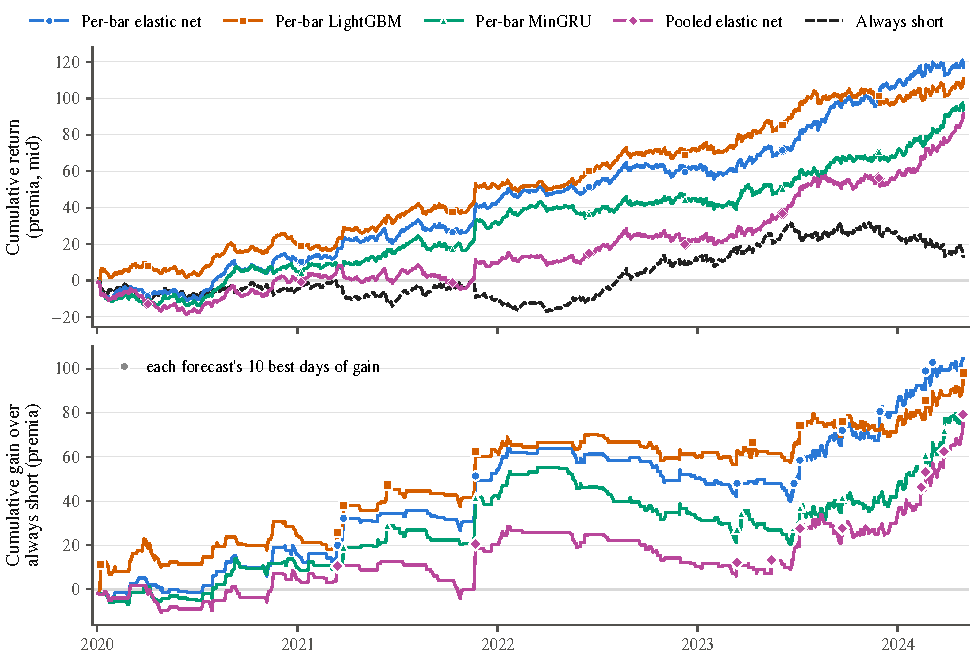
\includegraphics[width=\linewidth]{figures/rehaul_econ_cumpnl.pdf}
\caption{The closing trade over time, $q_t = \sign(s_t)$ at mid, for one forecast per family (all features) and
always short. Top: cumulative return $\sum_{u \le t} r_u$, in units of the straddle premium. Bottom: cumulative gain
over always short, $\sum_{u \le t} \bigl(r_u - r^{\mathrm{short}}_u\bigr)$; the markers are each forecast's 10
days of largest gain, each a day on which it bought and $R_t \ge 2.99$. The gain over the 866 days is
per-bar elastic net $+104.7$, per-bar LightGBM $+98.1$, per-bar MinGRU $+81.1$, pooled elastic net $+79.3$; without each forecast's 10 best days it is $+15.6$, $+2.4$, $-6.2$, $-6.3$. For 102 of the 112 forecasts of the model set the
gain is negative without their 10 best days.}
\label{fig:rh_econ_cumpnl}
\end{figure}


% E2: HAR + calendar -> all features within each family
% AUTO-GENERATED by writeup/make_rehaul_economics.py -- do not edit; re-run the script.
% Table E2 (outline 7.4): the full predictor set against the HAR benchmark
\ifdefined\rheNdays\else% AUTO-GENERATED by writeup/make_rehaul_economics.py -- do not edit; re-run the script.
% \rhe... macros for writeup/rehaul/07_economics.tex; values as in the rehaul_econ_* floats.
\providecommand{\rheShortSh}{}\renewcommand{\rheShortSh}{0.20}  % always short, Sharpe mid, 866 days
\providecommand{\rheShortShX}{}\renewcommand{\rheShortShX}{\ensuremath{-}0.27}  % always short, Sharpe crossed
\providecommand{\rheShortT}{}\renewcommand{\rheShortT}{0.43}  % always short, Newey-West t of the mean mid return
\providecommand{\rheShortHit}{}\renewcommand{\rheShortHit}{61.8}  % always short, hit rate %
\providecommand{\rheEnetSh}{}\renewcommand{\rheEnetSh}{1.92}  % per-bar enet all features, Sharpe mid
\providecommand{\rheEnetShX}{}\renewcommand{\rheEnetShX}{1.43}  % ... crossed
\providecommand{\rheEnetT}{}\renewcommand{\rheEnetT}{2.56}  % ... HAC t vs always short
\providecommand{\rheNNSh}{}\renewcommand{\rheNNSh}{1.53}  % MinGRU all features, Sharpe mid
\providecommand{\rheNNShX}{}\renewcommand{\rheNNShX}{1.05}  % ... crossed
\providecommand{\rheNNBaseSh}{}\renewcommand{\rheNNBaseSh}{1.04}  % MinGRU HAR + calendar, Sharpe mid
\providecommand{\rheNNBaseShX}{}\renewcommand{\rheNNBaseShX}{0.57}  % ... crossed
\providecommand{\rheSigVsShort}{}\renewcommand{\rheSigVsShort}{20}  % model-set forecasts with HAC t > 1.96 vs always short
\providecommand{\rhePairs}{}\renewcommand{\rhePairs}{51}  % HAR + cal. -> all features pairs in the model set
\providecommand{\rhePairsUp}{}\renewcommand{\rhePairsUp}{50}  % ... Sharpe mid higher with all features
\providecommand{\rhePairsSig}{}\renewcommand{\rhePairsSig}{4}  % ... HAC t > 1.96
\providecommand{\rhePairsMed}{}\renewcommand{\rhePairsMed}{\ensuremath{+}0.54}  % ... median dSharpe mid
\providecommand{\rheSzSignMed}{}\renewcommand{\rheSzSignMed}{0.92}  % sizing sign: model-set median Sharpe mid, 614 days
\providecommand{\rheSzClipMed}{}\renewcommand{\rheSzClipMed}{1.34}  % sizing clip: model-set median Sharpe mid, 614 days
\providecommand{\rheSzLfssMed}{}\renewcommand{\rheSzLfssMed}{1.12}  % sizing lfss: model-set median Sharpe mid, 614 days
\providecommand{\rheSzRankMed}{}\renewcommand{\rheSzRankMed}{1.34}  % sizing rank: model-set median Sharpe mid, 614 days
\providecommand{\rheSzShort}{}\renewcommand{\rheSzShort}{0.34}  % always short, Sharpe mid on the 614 sizing days
\providecommand{\rheSzClipBeats}{}\renewcommand{\rheSzClipBeats}{98}  % clip above sign(s), of 112 (mid)
\providecommand{\rheSzClipGain}{}\renewcommand{\rheSzClipGain}{\ensuremath{+}0.45}  % median clip - sign(s) Sharpe mid
\providecommand{\rheTailNeg}{}\renewcommand{\rheTailNeg}{102}  % model-set forecasts whose gain over short is < 0 without 10 best days
\fi
\begin{table}[tbp]
\centering
\small
\begin{threeparttable}
\caption{Sharpe ratios: HAR benchmark versus full predictor set}
\label{tab:rh_econ_allfeat}
\begin{tabular}{@{}lrrrr@{}}
\toprule
 & \multicolumn{2}{c}{$\SR$ at mid-quotes} & \multicolumn{2}{c}{$\Delta\SR$} \\
\cmidrule(lr){2-3}\cmidrule(l){4-5}
 & HAR benchmark & Full set & Mid-quotes & Bid--ask \\
\midrule
\multicolumn{5}{@{}l}{\textit{Panel A: Closing-interval models}} \\
\addlinespace[2pt]
Elastic net & $1.64$ & $1.93$ & $0.29^{\phantom{***}}$ & $0.29^{\phantom{***}}$ \\
 &  &  & $(1.34)^{\phantom{***}}$ & $(1.35)^{\phantom{***}}$ \\[2pt]
Lasso & $1.64$ & $1.76$ & $0.13^{\phantom{***}}$ & $0.13^{\phantom{***}}$ \\
 &  &  & $(1.47)^{\phantom{***}}$ & $(1.48)^{\phantom{***}}$ \\[2pt]
Ridge & $1.64$ & $1.51$ & $-0.13^{\phantom{***}}$ & $-0.13^{\phantom{***}}$ \\
 &  &  & $(0.09)^{\phantom{***}}$ & $(0.10)^{\phantom{***}}$ \\[2pt]
\addlinespace[4pt]
\multicolumn{5}{@{}l}{\textit{Panel B: Intraday models}} \\
\addlinespace[2pt]
Elastic net & $0.79$ & $1.91$ & $1.12^{\phantom{***}}$ & $1.13^{\phantom{***}}$ \\
 &  &  & $(1.21)^{\phantom{***}}$ & $(1.20)^{\phantom{***}}$ \\[2pt]
Lasso & $0.76$ & $1.56$ & $0.80^{\phantom{***}}$ & $0.80^{\phantom{***}}$ \\
 &  &  & $(1.19)^{\phantom{***}}$ & $(1.19)^{\phantom{***}}$ \\[2pt]
Ridge & $0.80$ & $1.73$ & $0.94^{\phantom{***}}$ & $0.94^{\phantom{***}}$ \\
 &  &  & $(1.12)^{\phantom{***}}$ & $(1.12)^{\phantom{***}}$ \\[2pt]
\addlinespace[4pt]
\multicolumn{5}{@{}l}{\textit{Panel C: Medians across pairs}} \\
\addlinespace[2pt]
LightGBM (\rheTreePairsEach) & $0.54$ & $1.40$ & $0.78^{\phantom{***}}$ & $0.77^{\phantom{***}}$ \\
 &  &  & $[0/15]^{\phantom{***}}$ & $[0/15]^{\phantom{***}}$ \\[2pt]
XGBoost (\rheTreePairsEach) & $0.57$ & $1.13$ & $0.51^{\phantom{***}}$ & $0.50^{\phantom{***}}$ \\
 &  &  & $[3/15]^{\phantom{***}}$ & $[3/15]^{\phantom{***}}$ \\[2pt]
Random forest (\rheTreePairsEach) & $0.26$ & $0.84$ & $0.50^{\phantom{***}}$ & $0.50^{\phantom{***}}$ \\
 &  &  & $[1/15]^{\phantom{***}}$ & $[1/15]^{\phantom{***}}$ \\[2pt]
All trees (\rheTreePairs) & $0.48$ & $1.15$ & $0.62^{\phantom{***}}$ & $0.61^{\phantom{***}}$ \\
 &  &  & $[4/45]^{\phantom{***}}$ & $[4/45]^{\phantom{***}}$ \\[2pt]
Model set (\rhePairs) & $0.50$ & $1.19$ & $0.62^{\phantom{***}}$ & $0.61^{\phantom{***}}$ \\
 &  &  & $[4/51]^{\phantom{***}}$ & $[4/51]^{\phantom{***}}$ \\[2pt]
\bottomrule
\end{tabular}
\begin{tablenotes}[flushleft]
\footnotesize
\item \textit{Notes:} Each pair is one model estimated on the HAR benchmark and on the full predictor set, with
everything else unchanged, over the out-of-sample period ($T_{\mathrm{oos}} = \rheNdays$ trading days). $\SR$ is the
annualized Sharpe ratio of the sign strategy; $\Delta\SR$ is the full-set minus the HAR-benchmark $\SR$, at
mid-quotes and at quoted bid/ask prices, with the HAC $t$-statistic on the daily return differential (Newey--West, $q_{\mathrm{NW}} = \rheHACLag$; Section~\ref{sec:rh_methods_tests}) in parentheses. On the HAR benchmark the three
closing-interval linear models hold the same position as the closing-interval OLS on every day, so they share its
$\SR$. Panel C gives medians across the closing-interval tree pairs (every hyperparameter specification in the model
set) and across all pairs of the \rheModelSetN{} forecasts of the model set, with the number of pairs whose
differential is significantly positive at the 5\% level in brackets (none is significantly negative at
that level). $^{*}$, $^{**}$ and $^{***}$ denote significance at the 10\%, 5\% and 1\% levels.
\end{tablenotes}
\end{threeparttable}
\end{table}


% E3: pooled vs per-bar (linear)
% AUTO-GENERATED by writeup/make_rehaul_economics.py -- do not edit; re-run the script.
% Table E3 (outline 7.4): closing-interval against intraday linear models
\ifdefined\rheNdays\else% AUTO-GENERATED by writeup/make_rehaul_economics.py -- do not edit; re-run the script.
% \rhe... macros for writeup/rehaul/07_economics.tex; values as in the rehaul_econ_* floats.
\providecommand{\rheShortSh}{}\renewcommand{\rheShortSh}{0.20}  % always short, Sharpe mid, 866 days
\providecommand{\rheShortShX}{}\renewcommand{\rheShortShX}{\ensuremath{-}0.27}  % always short, Sharpe crossed
\providecommand{\rheShortT}{}\renewcommand{\rheShortT}{0.43}  % always short, Newey-West t of the mean mid return
\providecommand{\rheShortHit}{}\renewcommand{\rheShortHit}{61.8}  % always short, hit rate %
\providecommand{\rheEnetSh}{}\renewcommand{\rheEnetSh}{1.92}  % per-bar enet all features, Sharpe mid
\providecommand{\rheEnetShX}{}\renewcommand{\rheEnetShX}{1.43}  % ... crossed
\providecommand{\rheEnetT}{}\renewcommand{\rheEnetT}{2.56}  % ... HAC t vs always short
\providecommand{\rheNNSh}{}\renewcommand{\rheNNSh}{1.53}  % MinGRU all features, Sharpe mid
\providecommand{\rheNNShX}{}\renewcommand{\rheNNShX}{1.05}  % ... crossed
\providecommand{\rheNNBaseSh}{}\renewcommand{\rheNNBaseSh}{1.04}  % MinGRU HAR + calendar, Sharpe mid
\providecommand{\rheNNBaseShX}{}\renewcommand{\rheNNBaseShX}{0.57}  % ... crossed
\providecommand{\rheSigVsShort}{}\renewcommand{\rheSigVsShort}{20}  % model-set forecasts with HAC t > 1.96 vs always short
\providecommand{\rhePairs}{}\renewcommand{\rhePairs}{51}  % HAR + cal. -> all features pairs in the model set
\providecommand{\rhePairsUp}{}\renewcommand{\rhePairsUp}{50}  % ... Sharpe mid higher with all features
\providecommand{\rhePairsSig}{}\renewcommand{\rhePairsSig}{4}  % ... HAC t > 1.96
\providecommand{\rhePairsMed}{}\renewcommand{\rhePairsMed}{\ensuremath{+}0.54}  % ... median dSharpe mid
\providecommand{\rheSzSignMed}{}\renewcommand{\rheSzSignMed}{0.92}  % sizing sign: model-set median Sharpe mid, 614 days
\providecommand{\rheSzClipMed}{}\renewcommand{\rheSzClipMed}{1.34}  % sizing clip: model-set median Sharpe mid, 614 days
\providecommand{\rheSzLfssMed}{}\renewcommand{\rheSzLfssMed}{1.12}  % sizing lfss: model-set median Sharpe mid, 614 days
\providecommand{\rheSzRankMed}{}\renewcommand{\rheSzRankMed}{1.34}  % sizing rank: model-set median Sharpe mid, 614 days
\providecommand{\rheSzShort}{}\renewcommand{\rheSzShort}{0.34}  % always short, Sharpe mid on the 614 sizing days
\providecommand{\rheSzClipBeats}{}\renewcommand{\rheSzClipBeats}{98}  % clip above sign(s), of 112 (mid)
\providecommand{\rheSzClipGain}{}\renewcommand{\rheSzClipGain}{\ensuremath{+}0.45}  % median clip - sign(s) Sharpe mid
\providecommand{\rheTailNeg}{}\renewcommand{\rheTailNeg}{102}  % model-set forecasts whose gain over short is < 0 without 10 best days
\fi
\begin{table}[tbp]
\centering
\small
\begin{threeparttable}
\caption{Closing-interval versus intraday models}
\label{tab:rh_econ_pooled}
\begin{tabular}{@{}lrrrrr@{}}
\toprule
 & \multicolumn{2}{c}{$\SR$ at mid-quotes} & \multicolumn{3}{c}{Intraday minus closing-interval} \\
\cmidrule(lr){2-3}\cmidrule(l){4-6}
 & Pooled & Closing & $\Delta\SR$, & $\Delta\SR$, & \\
 & intraday & interval & mid-quotes & bid--ask & $\Delta\QLIKE$ (\%) \\
\midrule
\multicolumn{6}{@{}l}{\textit{Panel A: Full predictor set}} \\
\addlinespace[2pt]
Elastic net & $1.85$ & $1.82$ & $0.03^{\phantom{***}}$ & $0.02^{\phantom{***}}$ & $27.1^{***}$ \\
 &  &  & $[0.947]^{\phantom{***}}$ & $[0.965]^{\phantom{***}}$ & $(4.14)^{\phantom{***}}$ \\[2pt]
Lasso & $1.73$ & $1.67$ & $0.06^{\phantom{***}}$ & $0.05^{\phantom{***}}$ & $37.9^{***}$ \\
 &  &  & $[0.891]^{\phantom{***}}$ & $[0.909]^{\phantom{***}}$ & $(4.84)^{\phantom{***}}$ \\[2pt]
Ridge & $1.64$ & $1.42$ & $0.22^{\phantom{***}}$ & $0.21^{\phantom{***}}$ & $27.5^{***}$ \\
 &  &  & $[0.584]^{\phantom{***}}$ & $[0.593]^{\phantom{***}}$ & $(4.18)^{\phantom{***}}$ \\[2pt]
\addlinespace[4pt]
\multicolumn{6}{@{}l}{\textit{Panel B: HAR benchmark}} \\
\addlinespace[2pt]
Elastic net & $0.95$ & $1.55$ & $-0.59^{\phantom{***}}$ & $-0.60^{\phantom{***}}$ & $14.1^{***}$ \\
 &  &  & $[0.134]^{\phantom{***}}$ & $[0.133]^{\phantom{***}}$ & $(2.86)^{\phantom{***}}$ \\[2pt]
Lasso & $0.95$ & $1.55$ & $-0.59^{\phantom{***}}$ & $-0.60^{\phantom{***}}$ & $14.1^{***}$ \\
 &  &  & $[0.134]^{\phantom{***}}$ & $[0.133]^{\phantom{***}}$ & $(2.86)^{\phantom{***}}$ \\[2pt]
Ridge & $0.95$ & $1.55$ & $-0.59^{\phantom{***}}$ & $-0.60^{\phantom{***}}$ & $14.1^{***}$ \\
 &  &  & $[0.134]^{\phantom{***}}$ & $[0.133]^{\phantom{***}}$ & $(2.86)^{\phantom{***}}$ \\[2pt]
\bottomrule
\end{tabular}
\begin{tablenotes}[flushleft]
\footnotesize
\item \textit{Notes:} Each row compares the closing-interval model with the intraday model of the same
estimator and predictor set, both with hyperparameters selected on a pre-sample, over the out-of-sample period
($T_{\mathrm{oos}} = \rheNdays$ trading days); the intraday model is evaluated on the closing interval. $\SR$
is the annualized Sharpe ratio of the sign strategy; $\Delta\SR$ is the intraday minus the closing-interval
$\SR$, at mid-quotes and at quoted bid/ask prices, with the $p$-value of the \citet{LedoitWolf2008} test of equal Sharpe ratios on the \rheSzDays{} post-warmup days, in brackets (Section~\ref{sec:rh_methods_tests}). $\Delta\QLIKE$ is the
intraday model's mean QLIKE relative to the closing-interval model's, in percent, with the Diebold--Mariano
statistic (Harvey--Leybourne--Newbold correction, Newey--West $q_{\mathrm{NW}} = \rheDMLag$) in parentheses; positive values favor
the closing-interval model, as in Table~\ref{tab:rh_axis2}. $^{*}$, $^{**}$ and $^{***}$ denote significance at the 10\%, 5\% and 1\% levels.
\end{tablenotes}
\end{threeparttable}
\end{table}


% Accuracy vs trade: the existing figure (writeup/make_fig_qlike_sharpe.py, \fqs... macros). The old paper places it
% in sections/results_close_option.tex:298-327; if the rehaul's results section also places it, keep one.
\ifdefined\fqsPairs\else% AUTO-GENERATED by writeup/make_fig_qlike_sharpe.py -- do not edit.
% Figure writeup/figures/fig_qlike_sharpe.pdf: QLIKE against Sharpe (mid), HAR + calendar vs all
% features, every model of results/close_master_table/paper_model_set.csv on both input sets
% (per-bar linear = the pre-tuned subpt_* rows; LSTMs excluded); numbers from master_table.csv
% and master_table_daily.parquet.  Changes are all features minus HAR + calendar, on the same days.
% DM: dm_test on the daily QLIKE difference; t: hac_inference.llsw_test on the daily mid-return
% difference (614 post-warmup days, bandwidth 33, fixed-b p); Sharpe changes: Ledoit-Wolf p;
% ES(c = 1): close_murphy_splits_headline.elementary on f / iv, y / iv.  Point estimates.
% pooled pairs: family pooled twin
\newcommand{\fqsPairs}{42}  % models on both input sets (pairs drawn)
\newcommand{\fqsPairsPerBarLinear}{3}  % of which per-bar linear (pre-tuned)
\newcommand{\fqsPairsPooled}{3}  % of which pooled 48-bar linear
\newcommand{\fqsPairsTree}{36}  % of which per-bar trees
\newcommand{\fqsPoints}{85}  % points drawn: both ends of every pair + the HAR + cal. OLS
\newcommand{\fqsDays}{866}  % trade days
\newcommand{\fqsQLower}{31}  % QLIKE lower with all features
\newcommand{\fqsQLowerSig}{3}  % ... and DM significant at 5 %
\newcommand{\fqsQHigher}{11}  % QLIKE higher with all features
\newcommand{\fqsQHigherSig}{0}  % ... and DM significant at 5 %
\newcommand{\fqsQLowerSigLagFourteen}{2}  % sensitivity: QLIKE lower, DM at lag 14 significant
\newcommand{\fqsQHigherSigLagFourteen}{0}  % sensitivity: QLIKE higher, DM at lag 14 significant
\newcommand{\fqsShHigher}{41}  % Sharpe (mid) higher with all features
\newcommand{\fqsShHigherSig}{6}  % ... and Ledoit-Wolf p < 0.05 (614 post-warmup days)
\newcommand{\fqsShLower}{1}  % Sharpe (mid) lower with all features
\newcommand{\fqsShLowerSig}{0}  % ... and Ledoit-Wolf p < 0.05 (614 post-warmup days)
\newcommand{\fqsQLowerShHigher}{30}  % both: QLIKE lower and Sharpe higher
\newcommand{\fqsMedDQ}{\ensuremath{-}0.0016}  % median QLIKE change (all features minus HAR + cal.)
\newcommand{\fqsMedDQPct}{\ensuremath{-}1.6}  % median QLIKE change, % of the HAR + cal. QLIKE
\newcommand{\fqsMedDSh}{\ensuremath{+}0.53}  % median Sharpe (mid) change
\newcommand{\fqsESLower}{29}  % elementary score at the threshold (c = 1) lower with all features
\newcommand{\fqsCorrES}{0.07}  % Pearson corr. across pairs: ES(c = 1) change vs HAC t of the P&L change
\newcommand{\fqsCorrQ}{0.12}  % Pearson corr. across pairs: QLIKE change vs HAC t of the P&L change
\newcommand{\fqsInShade}{4}  % all-features points in the shaded quadrant
\newcommand{\fqsInShadeBase}{3}  % HAR + cal. points in the shaded quadrant
\newcommand{\fqsOlsQ}{0.0967}  % QLIKE of the HAR + cal. OLS
\newcommand{\fqsOlsSh}{1.06}  % Sharpe (mid) of the HAR + cal. OLS
\newcommand{\fqsDMLag}{6}  % Newey-West lag of the DM statistic (the master table's)
\newcommand{\fqsHACS}{33}  % bandwidth S of the t of the mean P&L change (LLSW 2018, 614 post-warmup days)
\newcommand{\fqsSigPct}{5}  % two-sided level of the counts, %
\newcommand{\fqsQuadBetterBoth}{30}  % change figure: lower QLIKE, higher Sharpe
\newcommand{\fqsQuadShOnly}{11}  % change figure: higher QLIKE, higher Sharpe
\newcommand{\fqsQuadQOnly}{1}  % change figure: lower QLIKE, lower Sharpe
\newcommand{\fqsQuadWorseBoth}{0}  % change figure: higher QLIKE, lower Sharpe
\fi
% 2026-10-15 (user): parked -- non-standard figure; focus on legible tables
% \begin{figure}[tbp]
% \centering
% 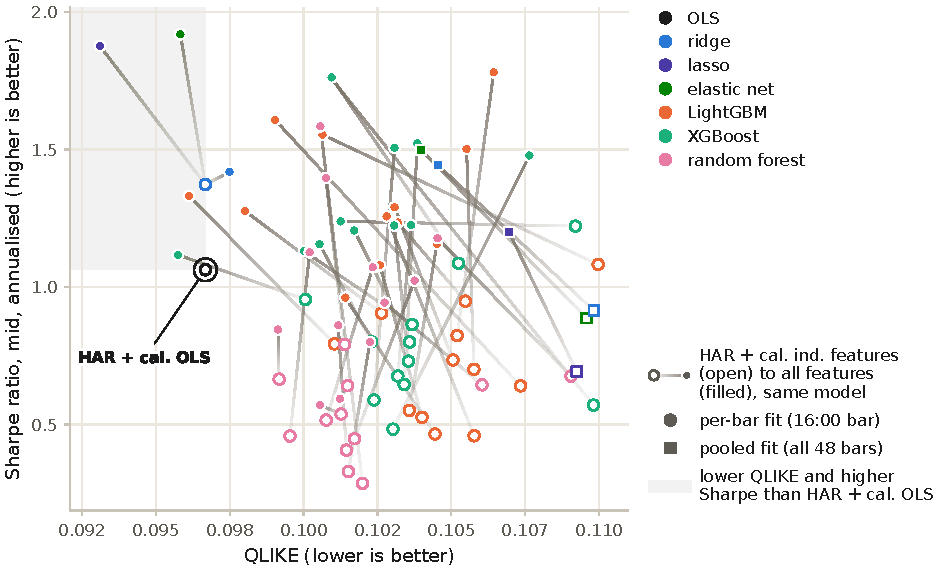
\includegraphics[width=\linewidth]{figures/fig_qlike_sharpe.pdf}
% % 2026-10-15 (notation pass): parked -- code jargon (trade, sign(s) Sharpe, per-bar, fits, HAR + calendar, all features, trade days); test wording
% % \caption{Accuracy against the trade: QLIKE and the $\sign(s)$ Sharpe ratio (mid) of the \fqsPairs{} models of the
% % model set fitted on both HAR + calendar (open markers) and all features (filled), \fqsDays{} trade days; each pair is
% % joined from its HAR + calendar end. Circles are per-bar fits and squares pooled fits; the colour marks the estimator.
% % Shaded: lower QLIKE and higher Sharpe ratio than the HAR + calendar OLS (QLIKE \fqsOlsQ, Sharpe \fqsOlsSh). All
% % features raise the Sharpe ratio for \fqsShHigher{} of the \fqsPairs{} models (\fqsShHigherSig{} significantly, by the
% % HAC $t$ of the daily return difference) and lower QLIKE for \fqsQLower{} (\fqsQLowerSig{} significantly, by
% % Diebold--Mariano), at \fqsSigPct\,\%.}
% \caption{Forecast accuracy and economic value. The figure plots the mean QLIKE loss against the annualized Sharpe
% ratio at mid-quotes, $\SR$, of the sign strategy for the \fqsPairs{} models of the model set that are estimated on both
% the HAR benchmark (open markers) and the full predictor set (filled markers), over the \fqsDays{} trading days of the
% out-of-sample period; a line joins the two ends of each pair. The sign strategy takes a delta-neutral at-the-money
% straddle position, entered at 15:30 ET and held to expiration: long ($q_t = +1$) or short ($q_t = -1$) as
% $q_t = \sign(s_t)$, where $s_t$ is the variance forecast minus the 15:30 implied variance. Circles denote
% closing-interval models and squares pooled intraday models; color identifies the estimator. The shaded quadrant
% contains lower QLIKE and higher $\SR$ than the closing-interval OLS on the HAR benchmark (QLIKE \fqsOlsQ, $\SR$
% \fqsOlsSh). The full predictor set raises $\SR$ for \fqsShHigher{} of the \fqsPairs{} models, \fqsShHigherSig{} of
% them significant at the \fqsSigPct\% level (HAC $t$-statistic on the daily return differential, Newey--West lag
% $q = \fqsHACLag$), and lowers QLIKE for \fqsQLower{}, \fqsQLowerSig{} of them significant at the \fqsSigPct\% level
% (Diebold--Mariano test with the Harvey--Leybourne--Newbold correction, Newey--West lag $q = \fqsDMLag$).}
% \label{fig:rh_econ_qlike_sharpe}
% \end{figure}

% E4: sizing rules
% AUTO-GENERATED by writeup/make_rehaul_economics.py -- do not edit; re-run the script.
% Table E4 (outline 7.4): position-sizing rules, scored exactly as the GUI (rows._score_sizes)
\ifdefined\rheNdays\else% AUTO-GENERATED by writeup/make_rehaul_economics.py -- do not edit; re-run the script.
% \rhe... macros for writeup/rehaul/07_economics.tex; values as in the rehaul_econ_* floats.
\providecommand{\rheShortSh}{}\renewcommand{\rheShortSh}{0.20}  % always short, Sharpe mid, 866 days
\providecommand{\rheShortShX}{}\renewcommand{\rheShortShX}{\ensuremath{-}0.27}  % always short, Sharpe crossed
\providecommand{\rheShortT}{}\renewcommand{\rheShortT}{0.43}  % always short, Newey-West t of the mean mid return
\providecommand{\rheShortHit}{}\renewcommand{\rheShortHit}{61.8}  % always short, hit rate %
\providecommand{\rheEnetSh}{}\renewcommand{\rheEnetSh}{1.92}  % per-bar enet all features, Sharpe mid
\providecommand{\rheEnetShX}{}\renewcommand{\rheEnetShX}{1.43}  % ... crossed
\providecommand{\rheEnetT}{}\renewcommand{\rheEnetT}{2.56}  % ... HAC t vs always short
\providecommand{\rheNNSh}{}\renewcommand{\rheNNSh}{1.53}  % MinGRU all features, Sharpe mid
\providecommand{\rheNNShX}{}\renewcommand{\rheNNShX}{1.05}  % ... crossed
\providecommand{\rheNNBaseSh}{}\renewcommand{\rheNNBaseSh}{1.04}  % MinGRU HAR + calendar, Sharpe mid
\providecommand{\rheNNBaseShX}{}\renewcommand{\rheNNBaseShX}{0.57}  % ... crossed
\providecommand{\rheSigVsShort}{}\renewcommand{\rheSigVsShort}{20}  % model-set forecasts with HAC t > 1.96 vs always short
\providecommand{\rhePairs}{}\renewcommand{\rhePairs}{51}  % HAR + cal. -> all features pairs in the model set
\providecommand{\rhePairsUp}{}\renewcommand{\rhePairsUp}{50}  % ... Sharpe mid higher with all features
\providecommand{\rhePairsSig}{}\renewcommand{\rhePairsSig}{4}  % ... HAC t > 1.96
\providecommand{\rhePairsMed}{}\renewcommand{\rhePairsMed}{\ensuremath{+}0.54}  % ... median dSharpe mid
\providecommand{\rheSzSignMed}{}\renewcommand{\rheSzSignMed}{0.92}  % sizing sign: model-set median Sharpe mid, 614 days
\providecommand{\rheSzClipMed}{}\renewcommand{\rheSzClipMed}{1.34}  % sizing clip: model-set median Sharpe mid, 614 days
\providecommand{\rheSzLfssMed}{}\renewcommand{\rheSzLfssMed}{1.12}  % sizing lfss: model-set median Sharpe mid, 614 days
\providecommand{\rheSzRankMed}{}\renewcommand{\rheSzRankMed}{1.34}  % sizing rank: model-set median Sharpe mid, 614 days
\providecommand{\rheSzShort}{}\renewcommand{\rheSzShort}{0.34}  % always short, Sharpe mid on the 614 sizing days
\providecommand{\rheSzClipBeats}{}\renewcommand{\rheSzClipBeats}{98}  % clip above sign(s), of 112 (mid)
\providecommand{\rheSzClipGain}{}\renewcommand{\rheSzClipGain}{\ensuremath{+}0.45}  % median clip - sign(s) Sharpe mid
\providecommand{\rheTailNeg}{}\renewcommand{\rheTailNeg}{102}  % model-set forecasts whose gain over short is < 0 without 10 best days
\fi
\begin{table}[tbp]
\centering
\small
\begin{threeparttable}
\caption{Sharpe ratios by position-sizing rule}
\label{tab:rh_econ_sizing}
\begin{tabular}{@{}lrrrr@{}}
\toprule
 & & Robust & Full long, & \\
 & Sign & clip & scaled short & Rank \\
\midrule
\multicolumn{5}{@{}l}{\textit{Panel A: $\SR$ at mid-quotes}} \\
\addlinespace[2pt]
Short straddle & \multicolumn{4}{c}{$0.32$ under every rule} \\
\multicolumn{5}{@{}l}{Pooled intraday models (\rhePoolNBars{} regular-hours intervals)} \\
\quad Ridge & $1.64$ & $1.79$ & $1.71$ & $1.78$ \\
\quad Lasso & $1.73$ & $1.89$ & $1.83$ & $1.79$ \\
\quad Elastic net & $1.85$ & $1.82$ & $1.86$ & $1.79$ \\
\quad LightGBM & $1.54$ & $1.50$ & $1.54$ & $1.56$ \\
\quad XGBoost & $1.54$ & $1.48$ & $1.56$ & $1.57$ \\
\quad Random forest & $1.88$ & $1.68$ & $1.87$ & $1.69$ \\
\multicolumn{5}{@{}l}{Closing-interval models (15:30--16:00 ET half hour)} \\
\quad OLS, HAR benchmark & $1.11$ & $1.49$ & $1.36$ & $1.58$ \\
\quad Ridge & $1.42$ & $1.61$ & $1.48$ & $1.66$ \\
\quad Lasso & $1.67$ & $1.66$ & $1.65$ & $1.75$ \\
\quad Elastic net & $1.82$ & $1.72$ & $1.74$ & $1.80$ \\
\addlinespace[2pt]
Model set, median & $0.84$ & $1.26$ & $1.06$ & $1.23$ \\
Model set, number above sign & -- & 82 & 83 & 80 \\
\addlinespace[4pt]
\multicolumn{5}{@{}l}{\textit{Panel B: $\SR$ at quoted bid/ask prices}} \\
\addlinespace[2pt]
Short straddle & \multicolumn{4}{c}{$-0.03$ under every rule} \\
\multicolumn{5}{@{}l}{Pooled intraday models (\rhePoolNBars{} regular-hours intervals)} \\
\quad Ridge & $1.29$ & $1.43$ & $1.40$ & $1.42$ \\
\quad Lasso & $1.37$ & $1.53$ & $1.53$ & $1.43$ \\
\quad Elastic net & $1.50$ & $1.46$ & $1.55$ & $1.43$ \\
\quad LightGBM & $1.18$ & $1.16$ & $1.24$ & $1.21$ \\
\quad XGBoost & $1.19$ & $1.14$ & $1.26$ & $1.22$ \\
\quad Random forest & $1.52$ & $1.33$ & $1.56$ & $1.34$ \\
\multicolumn{5}{@{}l}{Closing-interval models (15:30--16:00 ET half hour)} \\
\quad OLS, HAR benchmark & $0.76$ & $1.16$ & $1.06$ & $1.24$ \\
\quad Ridge & $1.08$ & $1.28$ & $1.17$ & $1.31$ \\
\quad Lasso & $1.32$ & $1.32$ & $1.35$ & $1.41$ \\
\quad Elastic net & $1.48$ & $1.39$ & $1.44$ & $1.45$ \\
\addlinespace[2pt]
Model set, median & $0.48$ & $0.93$ & $0.75$ & $0.89$ \\
Model set, number above sign & -- & 82 & 88 & 82 \\
\bottomrule
\end{tabular}
\begin{tablenotes}[flushleft]
\footnotesize
\item \textit{Notes:} Annualized Sharpe ratios of the straddle position $q_t$ under four sizing rules
(Section~\ref{sec:rh_econ_strategy}), each a function of $\hat\sigma^2_t - \mathrm{IV}^2_t$ and of its values on
earlier days $t' < t$ only; the sign rule is the sign strategy, and the short-straddle benchmark (Short straddle)
holds $q_t \equiv -1$ under every rule. The first \rheSzWarmup{} trading days of the out-of-sample period only estimate the
scale of $|\hat\sigma^2_{t'} - \mathrm{IV}^2_{t'}|$, so every rule is evaluated on the remaining \rheSzDays{} of
the \rheNdays{} trading days; at quoted bid/ask prices the bid--ask spread is paid on $|q_t|$ straddles. Every model except the OLS uses the full predictor set; the pooled
intraday models are those of Table~\ref{tab:rh_econ_control} (note a there). The last two rows of each panel give the median across the
\rheModelSetN{} forecasts of the model set and the number of them whose $\SR$ is above that of
their own sign strategy. Point estimates; no test is reported.
\end{tablenotes}
\end{threeparttable}
\end{table}

% 2026-10-15 (user): parked -- non-standard figure; focus on legible tables
% % AUTO-GENERATED by writeup/make_rehaul_economics.py -- do not edit; re-run the script.
\begin{figure}[tbp]
\centering
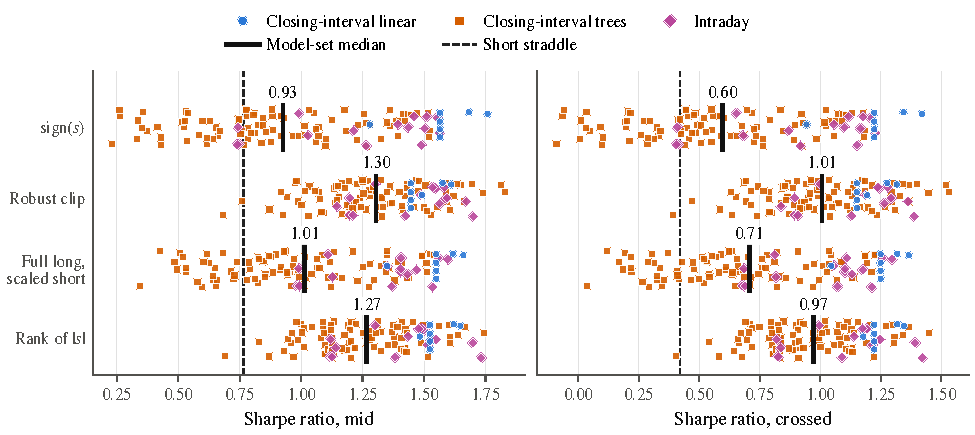
\includegraphics[width=\linewidth]{figures/rehaul_econ_sizing.pdf}
\caption{Sharpe ratio by sizing rule over the 94 forecasts of the model set, mid (left) and crossed (right),
on days 253--866. One marker per forecast, coloured by family and jittered vertically;
the bar and its label mark the model-set median (mid: 0.84, 1.26, 1.06, 1.23 for
the sign strategy, robust clip, full long / scaled short and rank of the absolute gap).
Dashed: the short-straddle benchmark ($0.32$ mid, $-0.03$ crossed). The
robust clip is above the sign strategy for 82 of the 94 forecasts at mid (median gain
$+0.45$). Rules and scoring as in Table~\ref{tab:rh_econ_sizing}.}
\label{fig:rh_econ_sizing}
\end{figure}


% Sharpe by year
% 2026-10-15 (user): parked -- non-standard figure; focus on legible tables
% % AUTO-GENERATED by writeup/make_rehaul_economics.py -- do not edit; re-run the script.
\begin{figure}[tbp]
\centering
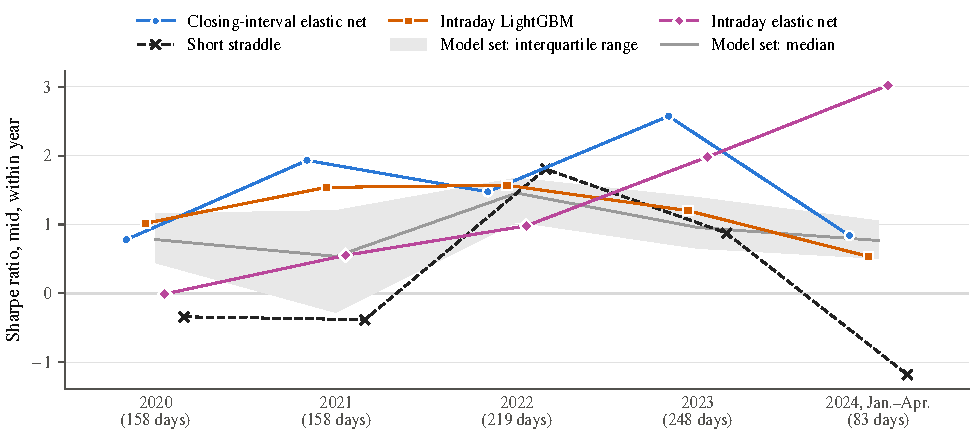
\includegraphics[width=\linewidth]{figures/rehaul_econ_byyear.pdf}
\caption{Sharpe ratio by calendar year at mid, $q_t = \sign(\hat\sigma^2_t - \mathrm{IV}^2_t)$, for the forecasts of
Figure~\ref{fig:rh_econ_cumpnl} and the short-straddle benchmark (2020 to 2024: $-0.34$, $-0.38$, $1.81$, $0.88$, $-1.18$); 2024 runs from
January to April. Each year's ratio is $\SR_y$ of Section~\ref{sec:rh_econ_measures}, scaled by the square root of that year's number of option days. Grey: the interquartile range
and median of the 112 forecasts of the model set (median $0.78$, $0.54$, $1.46$, $0.96$, $0.77$).}
\label{fig:rh_econ_byyear}
\end{figure}

